% Name: Stars and bars
% Description: Seven stars split by two bars into groups of 2, 4, and 1, one of the 36 ways to write 7 as an ordered sum of three counts that may be zero.
% Tags: stars and bars, combinations with repetition, counting, combinatorics

\usepackage{amsmath, amssymb}
\usetikzlibrary{decorations.pathreplacing}

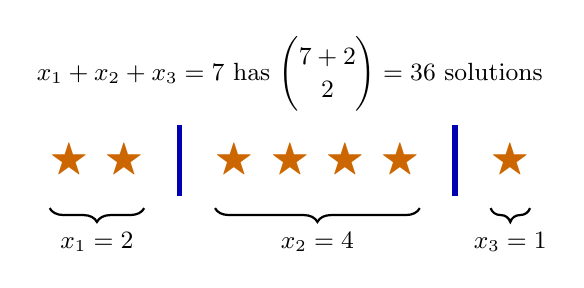
\begin{tikzpicture}[every node/.style={font=\small}]
  % Positions 0 to 8: stars at all but 2 and 7, which hold the bars
  \foreach \i in {0,1,3,4,5,6,8} \node[font=\Large, orange!80!black] at (0.7*\i,0) {$\bigstar$};
  \foreach \i in {2,7} \draw[line width=2pt, blue!70!black] (0.7*\i,-0.45) -- (0.7*\i,0.45);
  \draw[decorate, decoration={brace, mirror, amplitude=5pt}, thick] (-0.25,-0.6) -- node[below=5pt] {$x_1 = 2$} (0.95,-0.6);
  \draw[decorate, decoration={brace, mirror, amplitude=5pt}, thick] (1.85,-0.6) -- node[below=5pt] {$x_2 = 4$} (4.45,-0.6);
  \draw[decorate, decoration={brace, mirror, amplitude=5pt}, thick] (5.35,-0.6) -- node[below=5pt] {$x_3 = 1$} (5.85,-0.6);
  \node at (2.8,1.1) {$x_1 + x_2 + x_3 = 7$ has $\dbinom{7 + 2}{2} = 36$ solutions};
\end{tikzpicture}
